% -*- coding: utf-8 -*-

\chapter{Métodos de trabajo y herramientas}
\label{chap:methods}
\drop{E}{l} siguiente capítulo expone la metodología de trabajo escogida para
llevar a cabo el desarrollo del proyecto y describe las principales 
herramientas utilizadas para llevarlo a cabo.

\section{Pasos previos}
Antes de elegir una metodología concreta, conviene realizar un estudio rápido
de campo, para identificar cuáles son las partes que componen el sistema y para
definir \emph{a grosso modo} cuáles son las necesidades de información.

  \subsection{Estudio de campo}
  \label{sec:fieldStudy}
Como todo el mundo sabe, un restaurante es un \emph{``establecimiento público 
donde se sirven comidas y bebidas, mediante precio, para ser consumidas en el
mismo local''} \cite{bib:rae}.

Hoy en día existe una gran variedad de modalidades de servicio y tipos de
cocina.

    \subsubsection{Tipos de restaurantes}
  En cuanto a los tipos de establecimientos y fórmulas de restauranción, pueden
  distinguirse cinco clases\cite{bib:wiki}:
  \begin{itemize}
  \item \textbf{Tipo \emph{buffet}}. Los clientes escogen entre una serie de
  platos cocinados y dispuestos para el autoservicio. Normalmente se oferta
  una gran variedad de productos, pensados para todo tipo de clientes (figura
  \ref{fig:buffet}). El precio por comensal suele ser fijo, aunque también
  existe la modalidad de cobrar por peso o por tipo de platos consumidos.

  \begin{figure}[!h]
    \begin{center}
      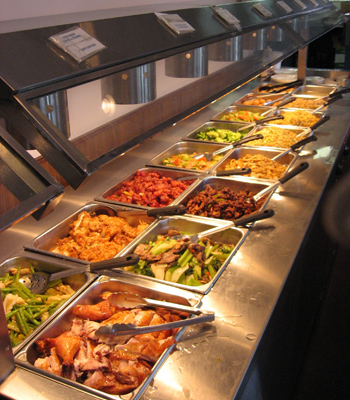
\includegraphics[width=0.5\textwidth]{buffet.png}
      \caption{Restaurante tipo \emph{buffet}.}
      \label{fig:buffet}
    \end{center}
  \end{figure}

  \item \textbf{Tipo \emph{fast food}}. Son restaurantes informales en los que
  se consumen platos de rápida preparación como: hamburguesas, perritos
  calientes, patatas fritas, pizzas o \emph{kebabs}, entre otros (figura
  \ref{fig:fastFood}). El usuarios de estos establecimientos busca la rapidez 
  del servicio, no la calidad nutricional o estética de los alimentos 
  servidos. Son, por lo general, los restaurantes más económicos.

  \begin{figure}[!h]
    \begin{center}
      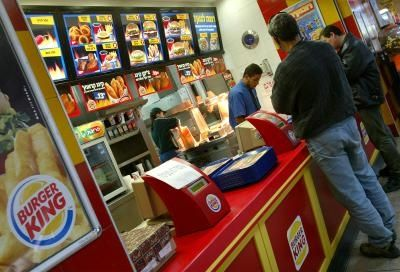
\includegraphics[width=0.6\textwidth]{fastFood.png}
      \caption{Restaurante de comida rápida.}
      \label{fig:fastFood}
    \end{center}
  \end{figure}

  \item \textbf{Tipo \emph{gourmet}}. Son restaurantes de más nivel, tanto por
  los productos preparan, como por la ambientación, la decoración y la atención
  que se ofrece (figura \ref{fig:gourmet}). Los pedidos son ``a la carta'' o
  escogidos de un ``menú'', por lo que los alimentos son cocinados al momento.
  Las mesas son atendidas por una serie de camareros dirigidos por un
  \emph{Maître}. El costo va en relación al servicio recibido y a la calidad de
  los platos consumidos.

  \begin{figure}[!h]
    \begin{center}
      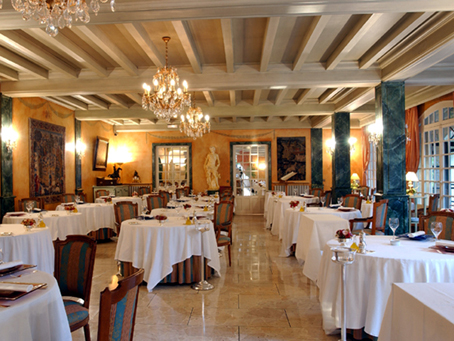
\includegraphics[width=0.7\textwidth]{gourmet.png}
      \caption{Restaurante tipo \emph{gourmet}.}
      \label{fig:gourmet}
    \end{center}
  \end{figure}

  \item \textbf{Tipo temático}. Son restaurantes que sirven exclusivamente
  productos típicos de un país o cultura. Suelen estar decorados y ambientados
  con motivos propios de la zona a la que representan (figura
  \ref{fig:themed}). Los tipos de cocina más populares en todo el mundo son: 
  la cocina italiana o la cocina china. Aunque también están muy extendidos 
  los restaurantes de cocina japonesa, brasileña, turca, india o tailandesa,
  entre otros.

  \begin{figure}[!h]
    \begin{center}
      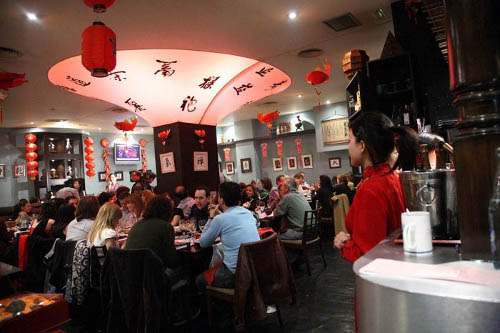
\includegraphics[width=0.7\textwidth]{themed.png}
      \caption{Restaurante con temática china.}
      \label{fig:themed}
    \end{center}
  \end{figure}

  \item \textbf{Tipo \emph{take away}}. Son similares a los restaurantes de
  comida rápida (\emph{fast food}), tanto en la rapidez del servicio, como en 
  el precio y en la calidad de los alimentos. El cliente se confecciona su 
  menú, eligiendo entre una serie de productos expuestos en vitrinas (frías y 
  calientes) (figura \ref{fig:takeAway}) y tiene la opción de consumirlos 
  dentro del establecimiento o puede llevárselos fuera. La vajilla y el menaje 
  que se usan son recipientes desechables.

  \begin{figure}[!h]
    \begin{center}
      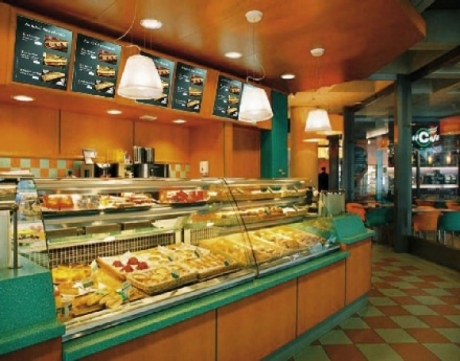
\includegraphics[width=0.6\textwidth]{takeAway.png}
      \caption{Restaurante tipo \emph{take away}.}
      \label{fig:takeAway}
    \end{center}
  \end{figure}

  \end{itemize}

  Las categorías citadas anteriormente no son excluyentes. Es decir, un
  restaurante puede estar clasificado en varias categorías. Por ejemplo, es muy
  común que los restaurantes de comida rápida (\emph{fast food}) ofrecezcan los
  servicios de restaurantes con comida para llevar (\emph{take away}). O los
  restaurantes temáticos pueden ofrecer un servicio tipo \emph{gourmet}.

    \subsubsection{Tipos de servicio}
  Según la forma de preparar, presentar y servir la comida y la bebida, un
  restaurante puede tener\cite{bib:wiki}:
  \begin{itemize}
  \item \textbf{Servicio francés}. La principal característica de este tipo de
  servicio es que el menú es elaborado en presencia del cliente (figura
  \ref{fig:frenchService}). Es decir, los ingredientes se traen de la cocina y
  se muestran al cliente para su inspección. A continuación, son devueltos a la
  cocina, donde se preparan. Y, una vez cocinados, el \emph{maître} prepara las
  raciones frente a la mesa, a gusto de cada comensal y las va sirviendo 
  siempre por la izquierda. Este tipo de servicio requiere gran habilidad por 
  parte del personal y por tanto resulta bastante caro. Es por ello que sólo 
  suele emplearse en los restaurantes de más alto nivel.

  \begin{figure}[!h]
    \begin{center}
      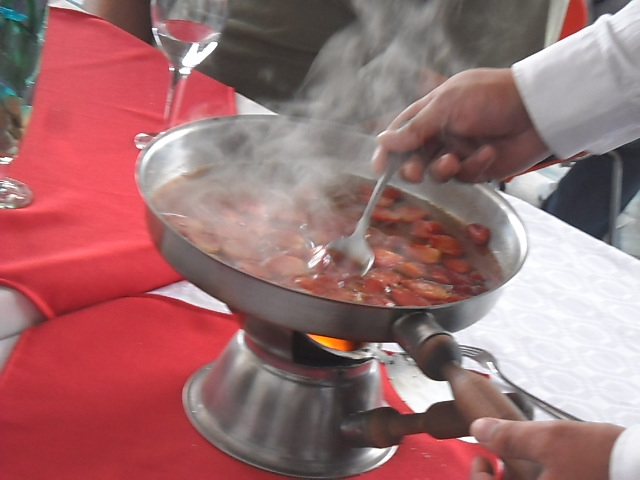
\includegraphics[width=0.6\textwidth]{frenchService.png}
      \caption{\emph{Maître} preparando raciones frente a una mesa. Típico del 
      \emph{servicio francés}.}
      \label{fig:frenchService}
    \end{center}
  \end{figure}

  \item \textbf{Servicio a la rusa}. Al sentarse, cada comensal encuentra 
  frente a él un plato vacío (el plato de servicio), sobre el que hay colocada 
  una servilleta. Y a izquierda y derecha se extienden los cubiertos que va a
  utilizar (salvo los del postre y alguno específico para carne o pescado)
  (figura \ref{fig:russianService}). Tras elegir aquello que va a tomar, se
  retira el plato de servicio y se van trayendo los platos encargados 
  siguiendo un orden específico (usualmente: sopas y entremeses, primeros 
  platos, segundos platos y postres). Cuando un comensal ha acabado con un 
  plato, el camarero lo retira y le trae el siguiente. Los platos son servidos 
  completamente preparados y presentados, por lo que no se requiere una 
  cualificación especial para los camareros. Esto ayuda a economizar y 
  dinamizar el servicio. En este caso, el \emph{maître} sólamente actúa como 
  jefe de sala, no sirve platos. Es el tipo de servicio de restaurante más 
  extendido.

  \begin{figure}[!h]
    \begin{center}
      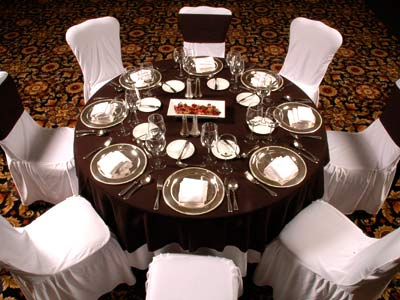
\includegraphics[width=0.6\textwidth]{russianService.png}
      \caption{Mesas equipadas conforme al \emph{servicio a la rusa}.}
      \label{fig:russianService}
    \end{center}
  \end{figure}

  \item \textbf{Servicio a la inglesa}. El comensal encuentra una disposición
  similar a la del \emph{servicio a la rusa}, con la diferencia de que, en este
  caso, el camarero sirve los alimentos desde una fuente o bandeja (siempre por
  la izquierda) (figura \ref{fig:englishService}). Como ocurría en el
  \emph{servicio francés}, el camarero va sirviendo sólamente el producto y la
  cantidad que el cliente solicita. En este tipo de servicio la presentación 
  del plato se pierde y es algo incómodo, tanto para el camarero como para el 
  comensal. Suele emplearse en algunos banquetes.

  \begin{figure}[!h]
    \begin{center}
      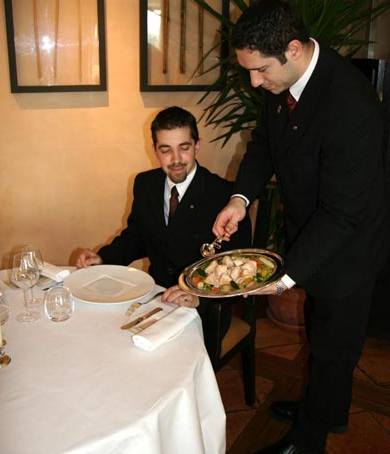
\includegraphics[width=0.4\textwidth]{englishService.png}
      \caption{Camarero sirviendo conforme al \emph{sercicio a la inglesa}.}
      \label{fig:englishService}
    \end{center}
  \end{figure}

  \item \textbf{Servicio americano}. Es una simplificación del \emph{servicio a
  la rusa} en el que se prima la rapidez. Los platos y las bebidas se sirven
  por la derecha y se retiran por la izquierda. Los alimentos que se sirven
  requieren poca preparación, tanto para su elaboración como para su servicio
  (figura \ref{fig:americanService}). Es el tipo de servicio más económico.

  \begin{figure}[!h]
    \begin{center}
      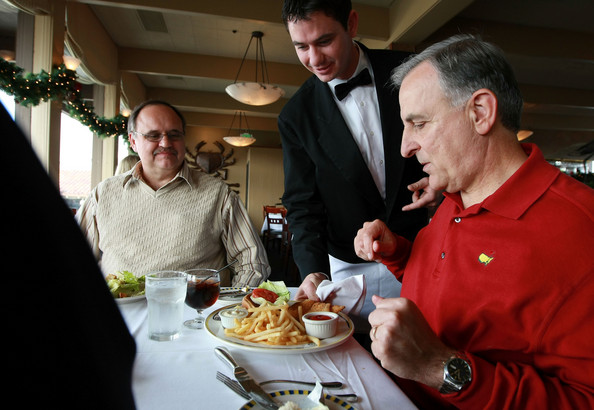
\includegraphics[width=0.6\textwidth]{americanService.png}
      \caption{Camarero sirviendo conforme al \emph{sercicio americano}.}
      \label{fig:americanService}
    \end{center}
  \end{figure}

  \end{itemize}

  Los restaurantes \emph{take away}, \emph{fast food} y \emph{buffet} suelen
  carecer de camareros y, por lo tanto, no pueden englobarse dentro de ninguno 
  de los tipos de servicio nombrados anteriormente. En cuanto a los 
  restaurantes de alta cocina (o \emph{gourmets}) y a los \emph{restaurantes 
  temáticos}, el tipo de servicio ofrecido está directamente relacionado con 
  el nivel del establecimiento.

  \subsection{Consideraciones del escenario}
    \subsubsection{Restaurante tipo para el \acs{PFC}}
  El presente \acs{PFC} va - en principio - orientado a restaurantes de tipo
  \emph{gourmet} o \emph{temático}, que son restaurantes que cuentan con
  servicio de camareros y disponen de una carta de productos. Además, el
  restaurante debe contar con un punto de  control de entrada o
  \textbf{recibidor}, que debe estar custodiado por un \emph{maître}. Este se
  encargará de atender a los clientes que entran y les procurará asiento.

  Un trabajo futuro podría consistir en adaptar el sistema para restaurantes 
  de tipo \emph{fast food} o \emph{take away} (que no tienen control de 
  entrada). Para restaurantes tipo \emph{buffet}, en cambio, no tendría
  sentido automatizar los pedidos, puesto que no existen.

  Por otro lado, el tipo de servicio ofrecido no va a afectar al funcionamiento
  del sistema a desarrollar.

    \subsubsection{Necesidades de información}
  En primer lugar, el sistema debe ser capaz de gestionar la información
  típica con la que trabajan la mayor parte de las aplicaciones de
  restauración que existen hoy en día. Es decir, debe gestionar: la lista
  de productos puestos a la venta; el precio, los impuestos y los
  descuentos de cada uno de ellos; el estado, la lista de pedidos y la
  facturación de cada mesa; etc.

  Por otro lado, el sistema está encaminado a que el cliente pueda 
  identificarse a través de su dispositivo móvil, para: realizar
  pedidos desde su mesa, recibir descuentos y recomendaciones según su
  historial y poder realizar pagos mediante \acs{NFC}. Por lo que otro de los
  objetos a tener en cuenta \textbf{son los clientes} y el historial que dejan
  a través de sus pedidos y accesos al local.

    \subsubsection{Elección de tecnologías}
  El sistema estará formado por varias aplicaciones que se comunican entre sí.
  Para gestionar los datos con los que trabajan las aplicaciones del
  restaurante, se contará con una \textbf{base de datos} distribuida, a la que
  se accederá a través de \textbf{servicios web}. Con esto se conseguirá la
  sincronización y persistencia de los datos con los que se están trabajando
  en cada momento.

  El uso combinado de la \textbf{tecnología \acs{NFC}} con el de las
  \textbf{etiquetas \acs{RFID}}, permitirá al cliente interactuar con los
  elementos del restaurantes con el simple hecho de acercar su dispositivo
  móvil a unas u otras etiquetas.

  La tecnología inalámbrica móvil que ofrece mayores posibilidades a la hora
  de comunicar el dispositivo móvil con los equipos fijos del restaurante es
  la tecnología \acs{WiFi}. No obstante, el único dispositivo móvil con el que
  se cuenta (\emph{\textbf{Nokia 6131 \acs{NFC}}}, facilitado por el
  \textbf{\emph{grupo \acs{MAmI}\footnote{Grupo de investigación de la
  \acs{UCLM} que tiene como principal objetivo adaptar las tecnologías para 
  modelar contextos en los que se minimice o desaparezca la interacción del 
  usuario de tal manera que éste perciba la asistencia del entorno que le 
  rodea.}}} y que incluye la tecnología \acs{NFC}) no
  dispone esa tecnología. Por ello, se opta por echar mano de otra de las
  tecnologías inalámbricas más extendidas entre los dispositivos móviles, la
  \textbf{tecnología \emph{Bluetooth}}.

  \subsection{Aplicación de los servicios web}
    \subsubsection{Gestión de los datos de un restaurante}
  El sistema informático a desarrollar va a estar formado por varias
  aplicaciones. Estas aplicaciones van a tener que compartir los datos con
  los que operan. Para garantizar la sincronización y la integridad de los
  datos, se propone crear un servicio web, independiente a las demás
  aplicaciones, que se encargue de gestionar los accesos a la base de datos
  que contiene, valga la redundancia, dichos datos.

    \subsubsection{\emph{ASP .NET}}
%%%%%%%%%%%%%%%%%%%%%%%%%%%%%%%%%

    \subsubsection{Base de datos \emph{MySQL}}
%%%%%%%%%%%%%%%%%%%%%%%%%%%%%%%%%

  \subsection{Aplicación de la tecnología \acs{NFC}}
    \subsubsection{Introducción de la tecnología \acs{NFC} en el entorno}
  La introducción de la tecnología \acs{NFC} en un restaurante tiene por
  objetivo identificar automáticamente a los clientes a su entrada. A partir de
  su identificación, el restaurante puede ofrecerles servicios como:
  realización de pedidos mediante una carta de etiquetas \acs{RFID} (desde la
  mesa y sin necesidad de llamar al camarero), recomendaciones a medida
  (calculadas a partir del histórico de pedidos del cliente en el restaurante),
  descuentos por fidelización (los clientes recibirán descuentos periódicos
  después   de varias visitas) y pago a través del móvil. Todos estos servicios
  son posibles gracias a la combinación de la tecnología \acs{NFC} con alguna
  tecnología inalámbrica de mayor alcance (como \acs{WiFi} o \emph{Bluetooth})
  puesto que el cliente debe comunicarse también con los ordenadores del
  restaurante.
  
    \subsubsection{Nokia 6131 \acs{NFC}}
  Hoy en día el número de
%%%%%%%%%%%%%%%%%%%%%%%%%%%%%%%%%%%%%%%
  %http://www.nfcon.es/2012/03/23/lista-de-telefonos-moviles-smartphones-con-nfc/

  % Móvil de MAmI
  % Nokia 6131NFC
  % Soporte Java
  % JSR-257

  \subsection{Aplicación de la tecnología Bluetooth}
%%%%%%%%%%%%%%%%%%%%%%%%%%%
    \subsubsection{Introducción de la tecnología \emph{Bluetooth} en el
  entorno}
%%%%%%%%%%%%%%%%%%%%%%%%%%%
    \subsubsection{Comunicación en serie}
%%%%%%%%%%%%%%%%%%%%%%%%%%%

\section{Metodología de trabajo}
\label{sec:workingMethodology}
Después de los pasos citados anteriormente se decide, para abordar el
desarrollo del proyecto, optar por una adaptación de la metodología de 
\emph{\textbf{prototipado incremental}}.

  \subsection{Prototipado incremental}
El objetivo de este \acs{PFC} es la creación del prototipo de un sistema.
Según \cite{bib:software_engineering}, \emph{``un prototipo puede definirse
como  un modelo parcial ejecutable de un sistema de software''.} Por lo tanto, 
no se pretende crear un producto final comercializable, sino más bien, un
modelo parcial de un sistema que ayude a comprender cómo funcionaría la
implantación de este sistema bajo las condiciones de un entorno real.

Pero, como su nombre indica, se pretende crear un sistema, es decir, un
\emph{``conjunto de cosas que relacionadas entre sí ordenadamente contribuyen 
a determinado objeto''}\cite{bib:rae}. Por lo que la creación de este prototipo
deberá hacerse teniendo en cuenta que está formado por otros prototipos más 
elementales que están relacionados entre sí.

Según \cite{bib:software_engineering}, el prototipado incremental \emph{``
se basa en la generación de varios modelos parciales ejecutables del sistema 
antes de proceder a la implementación (durante la especificación y durante el 
diseño) con el fin de evaluar sus características y poder obtener al final el 
sistema implementado.''.}

Cada nuevo ``modelo parcial'' se obtendrá a partir del ``modelo parcial''
anterior (validado por los usuarios y/o los analistas) junto con la
introducción de nuevos elementos funcionales del sistema. Esto se repetirá
hasta tener el sistema completo implementado (figura
\ref{fig:incremental_prototyping}).

\begin{figure}[!h]
  \begin{center}
    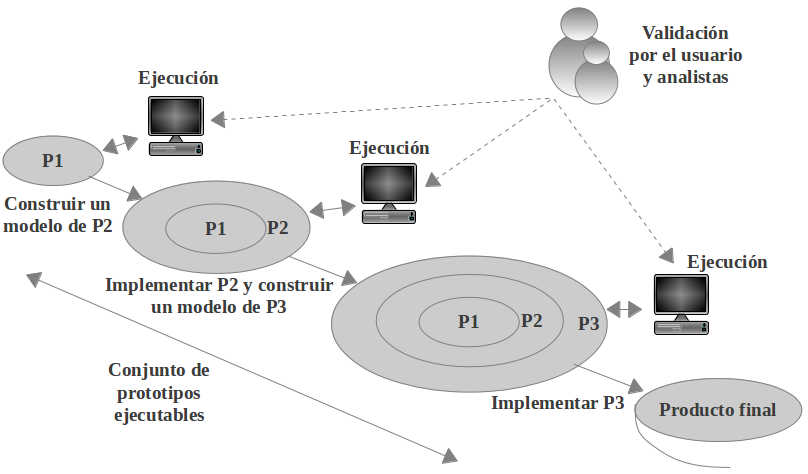
\includegraphics[width=0.9\textwidth]{incremental_prototyping.png}
    \caption{Ciclo de vida del prototipado incremental.}
    \label{fig:incremental_prototyping}
  \end{center}
\end{figure}

Como el sistema está formado por varios prototipos, habrá ``modelos parciales''
en los que estén involucrados varios de estos prototipos y otros en los que
sólo se implementen funcionalidades propias de uno de los prototipos del
sistema.

%.pdf "Prototipado incremental"

%Para \cite{bib:incremental_prototyping}, las fases típicas del ciclo de vida
%para el \emph{prototipado incremental} son las siguientes (figura
%\ref{fig:incremental_prototyping}):
%
%\begin{figure}[!h]
%  \begin{center}
%    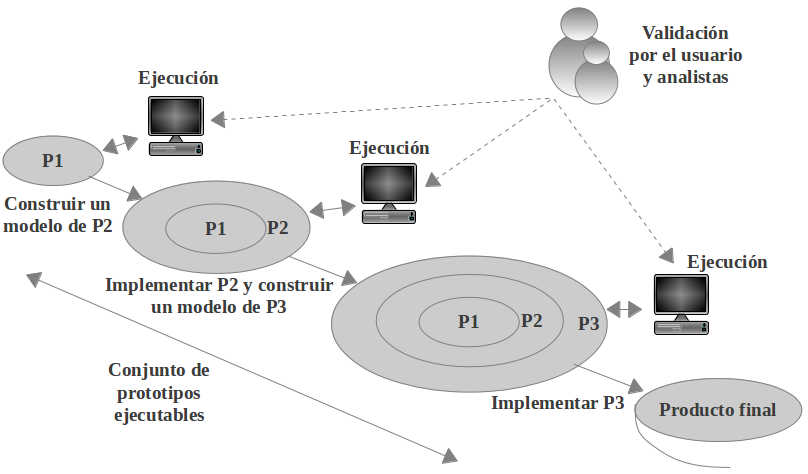
\includegraphics[width=0.8\textwidth]{incremental_prototyping.png}
%    \caption{Ciclo de vida del prototipado incremental.}
%    \label{fig:incremental_prototyping}
%  \end{center}
%\end{figure}
%
%\begin{enumerate}
%\item \textbf{Requisitos del proyecto}. Esta fase afecta al proyecto en su
%conjunto e incluye acciones como: el enunciado del problema que se
%pretende resolver, diagramas de clases y diccionarios y modelos de datos.
%\item \textbf{Requisitos del módulo}. Se definen los requisitos (software y
%hardware) de uno de los módulos o subsistemas.
%\item \textbf{Diseño del módulo}. Fase de diseño de la funcionalidad básica 
%del módulo que se está resolviendo. Se identifican qué clases son propias de %%este módulo, cuáles son compartidas y cuáles de las de otros módulos nos
%proporcionan datos e información.
%\item \textbf{Codificación A}. Implementación básica correspondiente a las
%funcionalidades definidas en \emph{diseño del módulo}.
%\item \textbf{Validación}. Se pone a prueba el prototipo obtenido en la
%\emph{codificación A} y se evalúan los resultados obtenidos durante la
%ejecución.
%\item \textbf{Diseño avanzado}. Se diseñan las funcionalidades complejas no
%implementadas en \emph{Diseño del módulo}.
%\item \textbf{codificación B}. Implementación de las funcionalidades
%avanzadas diseñadas en \emph{diseño avanzado}.
%\item \textbf{Validación}. Se pone a prueba el prototipo obtenido en la
%\emph{codificación B}.
%\end{enumerate}

%Una vez completado este último paso, se entrega el módulo a producción y se
%realiza una última revisión relacionada con garantizar (entre otras): la 
%integración del módulo dentro del sistema, la modularidad o la usabilidad
%del módulo implementado.
%
%Para el caso que nos ocupa, se tendrá un módulo por cada elemento que forme
%el sistema.

  \subsection{Estructura general del sistema}
Tras el estudio de campo realizado, las consideraciones del escenario y la
descripción de las principales tecnologías que se van a emplear, se propone
el siguiente escenario (figura \ref{fig:scenario}) como el \emph{escenario
tipo} sobre el cual implementar el sistema.

\begin{figure}[!h]
  \begin{center}
    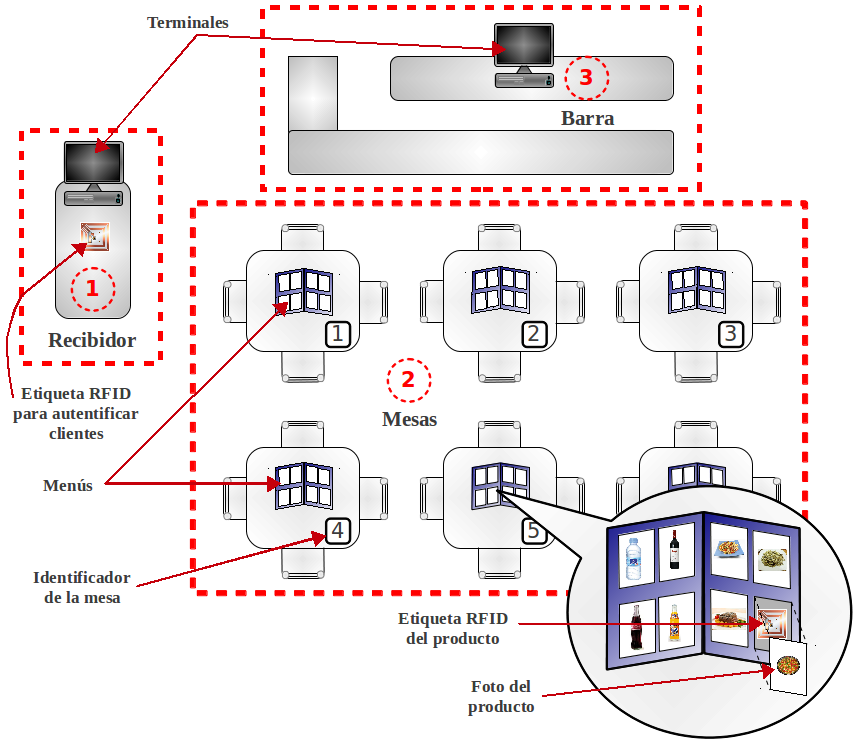
\includegraphics[width=1\textwidth]{scenario.png}
    \caption{Escenario tipo del sistema.}
    \label{fig:scenario}
  \end{center}
\end{figure}

    \subsubsection{El restaurante}
  El restaurante dispondrá de tres zonas claramente definidas:
  \begin{enumerate}
  \item El \textbf{recibidor}. Es la zona por la que se accede al salón del
  restaurante. Estará regentada por un maître que, ayudado por un terminal,
  registrará la entrada y salida de clientes y la asignación de mesas.
  Además, el maître también se encargará de gestionar los cobros mediante
  \acs{NFC}.
  \item Las \textbf{mesas}. Cada mesa tendrá un identificador único que la
  diferencie de las demás mesas. Este identificador servirá para poder
  asociar al cliente registrado con la mesa que está ocupando. Cada mesa
  contará con una carta de productos compuesta por varias etiquetas
  \acs{RFID}. Cada etiqueta contendrá la información de un producto. Esto 
  permitirá al cliente elaborar la lista de productos para un pedido
  mediante su dispositivo móbil \acs{NFC}.
  \item La \textbf{barra}. Es la zona donde se reciben los pedidos. Algunos
  podrán ser atendidos sobre la marcha por los camareros y otros necesitarán
  ser elaborados antes por los cocineros. Todos los pedidos recibidos serán
  registrados en un terminal, de manera que se vaya generando una lista de
  pedidos por cada mesa. Esto ayudará a la gestión del estado de dichos 
  pedidos y a facturación (en conjunto) de los mismos.
  \end{enumerate}

  Tanto el terminal del recibidor como el terminal de la barra dispondrán
  de un punto de conexión \emph{Bluetooth}, para posibilitar la comunicación
  con los dispositivos móviles de los clientes.

  Por otro lado, uno de los terminales citados u otro terminal distinto (que
  no tiene porqué estar en el mismo establecimiento) se encargará de hospedar
  al \textbf{servicio web}, que es la entidad a la que recurren los otros
  terminales para actualizar sus datos.

  Con la \textbf{base de datos} ocurre lo mismo. Puede encontrarse en uno de
  los terminales del restaurante, en el mismo terminal que el servicio web o
  en un terminal distinto. Se encargará de garantizar la persistencia de los
  datos generados por el sistema.

%  La figura \ref{fig:structure} muestra la estructura general del sistema.

%  \begin{figure}[!h]
%    \begin{center}
%      \includegraphics[width=0.8\textwidth]{structure.png}
%      \caption{Estructura general del sistema.}
%      \label{fig:structure}
%    \end{center}
%  \end{figure}

    \subsubsection{Los clientes}
    \label{subsubsec:clients}
  Habrá dos tipos de clientes:
  \begin{enumerate}
  \item \emph{\textbf{Clientes \acs{NFC}}}. Son potenciales \emph{clientes
  \acs{NFC}} los clientes que tienen un móvil con la tecnología \acs{NFC} y
  \emph{Bluetooth}. La tecnología \acs{NFC} les permitirá realizar acciones
  como: comunicar su llegada o su salida, pagar o elaborar una lista de
  productos para un pedido; con el simple gesto de tocar unas u otras
  etiquetas \acs{RFID}. El \emph{Bluetooth} por su parte, permitirá la
  comunicación entre el dispositivo del cliente y los terminales del
  restaurante para, por ejemplo: mandar sus datos personales, recibir
  recomendaciones, enviar pedidos o recibir el resumen de su factura.
  \item \emph{\textbf{Clientes normales}}. Los clientes que no disponen
  de un dispositivo móvil con las características de los \emph{clientes
  \acs{NFC}} o que simplemente no hacen uso de él. Su conducta para con
  el restaurante será la misma que la que sigue comunmente en este tipo
  de establecimientos: le solicita una mesa al maître, se sienta, le
  pide al camarero lo que desea tomar, se lo sirven, lo consume, solicita
  la cuenta, paga y se va. Este tipo de clientes no podrá recibir
  recomendaciones y no disfrutará de los descuentos que sí se le aplican
  a los \emph{clientes \acs{NFC}}.
  \end{enumerate}

  \subsection{Fases del prototipo}
Como se dijo anteriormente, el prototipo del sistema se construirá de forma
incremental a partir de varias iteraciones en las que se irán añadiendo
nuevas funcionalidades al sistema elemental (de la primera iteración). Las
iteraciones propuestas para el desarrollo del sistema son las siguientes:
\begin{enumerate}
\item Prototipo inicial de los servicios web y la base de datos.
\item Prototipo inicial del recibidor y conexión con los servicios web.
\item Prototipo inicial de la barra y conexión con los servicios web.
\item Prototipo inicial de la aplicación móvil.
\item Conexiones \emph{Bluetooth} entre el prototipo del móvil y el del
\emph{recibidor}.
\item Conexiones \emph{Bluetooth} entre el prototipo del móvil y el de la
\emph{barra}.
\item Sistema recomendador en el servicio web. Esto afectará al prototipo del 
recibidor y al prototipo de la aplicación móvil.
\end{enumerate}

%Como se dijo anteriormente, el prototipo del sistema que se pretende
%construir estará compuesto por los prototipos de los elementos que los forman.
%Y estos prototipos van seguir las fases de los ``módulos'' del ciclo
%de vida del \emph{prototipado incremental}. Por lo tanto, se va a contar con
%tres módulos:
%\begin{itemize}
%  \item \textbf{Servicio web y base de datos}.
%  \item \textbf{Aplicación del recibidor}.
%  \item \textbf{Aplicación de la barra}.
%\end{itemize}
%Las fases de \emph{diseño del módulo}, \emph{codificación A} y
%\emph{validación} van a coincidir con la definición, el desarrollo y las
%pruebas realizadas para la funcionalidad básica de este módulo; es decir, la
%funcionalidad común con los gestores típicos que hay en los restaurantes. Y 
%las fases de \emph{diseño avanzado}, \emph{codificación B} y la última
%\emph{validación}; van a coincidir con la definición, el desarrollo y las 
%pruebas realizadas para la funcionalidad avanzada. Esto es, la funcionalidad
%relativa a las operaciones relacionadas con el uso de la tecnología \acs{NFC} y
%\emph{Bluetooth}.

%Explicar donde queda la aplicación móvil y que entre la elaboración del
%primer modelo (Codificación A) y el segundo (Codificación B) debe haberse
%definido la aplicación del móvil (para todos los módulos).

\section{Herramientas}
En esta sección se citan las herramientas que han sido utilizadas para el 
desarrollo de este \acs{PFC}.

  \subsection{Diagramas \acs{UML}}
  Para cubrir la fase de análisis de requisitos y diseño de cada una de las
  iteraciones propuestas se ha echado mano del \emph{\textbf{Visual Paradigm
  for \acs{UML}}}, que es una herramienta \emph{case} de especificaciones
  \acs{UML}, desarrollado por la empresa \emph{Visual Paradigm International}.

  Con este programa se han realizado los diagramas de casos de uso, los de
  clases, los de despliegue, los de comunicación y los de secuencia. Es decir,
  todos los diagramas que definen la forma en la que está estructurado el
  sistema y la forma en que se comporta.

  La versión utilizada ha sido la \emph{8.3} de la \emph{Community Edition} y
  ha sido necesario pedir una licencia para uso \emph{no comercial}.

  \subsection{Lenguajes de programación}
  El código de los distintos elementos que forman el sistema ha sido
  implementado utilizando tres lenguajes de programación:

  \begin{itemize} 
  \item \textbf{C\#}.
  Es un lenguaje de programación orientada a objetos
  \acs{OO} desarrollado y estandarizado por \emph{Microsoft} como parte de
  su plataforma \emph{.NET}.

  Con este lenguaje se ha desarrollado la aplicación del \emph{recibidor} y
  la aplicación de la \emph{barra}.

  Además, se han utilizado la librería externa \emph{InTheHand.Net}, que
  posibilita las conexiones \emph{Bluetooth} de las aplicaciones implementadas
  en \emph{C\#} con los dispositivos móviles.

  \item \textbf{ASP.NET}.
  En realidad \emph{\acs{ASP}.NET} no puede 
  considerarse un lenguaje de programación, más bien es un \emph{framework} 
  que se utiliza para la construcción de sitios web dinámicos, aplicaciones 
  web o servicios web \acs{XML}. \emph{ASP.NET} está construido sobre el
  \emph{Common Language Runtime}, lo que permite a los programadores escribir 
  código \emph{ASP.NET} utilizando cualquier lenguaje admitido por el
  \emph{framework} de \emph{.NET}, como por ejemplo, el propio \emph{C\#}.

  Los servicios web han sido implementados utilizando el \emph{framework}
  \emph{ASP.NET}.

  Además, para poder acceder a la base de datos, se ha utilizado una librería
  externa a \emph{C\#} llamada \emph{MySql.Data}.

  \item \textbf{SQL}.
  \acs{SQL} es un lenguaje declarativo de acceso a bases de
  datos relacionales que permite especificar distintos tipos de operaciones
  sobre estas.

  En este caso la base de datos a la que se accede está montada sobre un
  \acs{SGBD} \emph{MySQL}. Esta base de datos almacena todos los datos de
  interés con los que trabajan las dos aplicaciones del restaurante
  (\emph{recibidor} y \emph{barra}).

  \item \textbf{Java Micro Edition}.
  Es una especificación de un subconjunto de la
  plataforma \emph{Java} orientada a proveer una colección certificada de
  \acs{API}s de desarrollo de software para dispositivos con recursos
  restringidos, como son los dispositivos móviles.

  \acs{JavaME} fue desarrollado mediante el Java Community Process bajo la 
  especificación \emph{JSR 68}. La evolución de la plataforma ha propiciado el 
  abandono de las Java Specification Request (peticiones de especificación 
  para Java) en favor de JSRs separadas para las distintas versiones de JavaME.

  Por ejemplo, para el desarrollo de la aplicación móvil se han utilizado
  principalmente dos \acs{JSR}s:
    \begin{itemize}
    \item \textbf{JSR-82}. Que implementa las funcionalidades
    propias de las comunicaciones vía \emph{Bluetooth} entre dispositivos.
    \item \textbf{JSR-257}. Que implementa las funcionalidades propias
    de las comunicaciones \acs{NFC}.
    \end{itemize}

  Además de estas, también se ha hecho uso de la librería
  \emph{kxml2-min-2.3.0} que permite construir y parsear documentos o cadenas 
  expresados en \acs{XML}.

  \item \textbf{XML}.
  Es un lenguaje de marcar desarrollado por el
  World Wide Web Consortium (\acs{W3C}). Permite definir la gramática de
  lenguajes específicos para estructurar documentos grandes. A diferencia de
  otros lenguajes, \emph{XML} da soporte a bases de datos, siendo útil cuando
  varias aplicaciones se deben comunicar entre sí o integrar información.

  En este caso, se utiliza \acs{XML} para mandar información estructurada 
  entre las aplicaciones del restaurante y los servicios web (a través de la
  red) y entre los dispositivos móviles y las aplicaciones del restaurante 
  (esta vez vía \emph{Bluetooth}).
  \end{itemize}

  \subsection{Aplicaciones de desarrollo}
  Para implementar las distintas aplicaciones que conforman el sistema se
  ha hecho uso de las siguientes herramientas de desarrollo:
  
  \begin{itemize}
    \item \textbf{Microsoft Visual Studio 2010}.
    Es un entorno de desarrollo integrado (\acs{IDE}) para sistemas operativos
    \emph{Windows}. Soporta lenguajes de programación como \emph{Visual C++},
    \emph{Visual C\#}, \emph{Visual J\#}, \emph{Visual Basic .NET} y
    entornos de desarrollo web como \emph{ASP.NET}, aunque actualmente
    se han desarrollado extensiones para muchos otros.

    Este \acs{IDE} se ha utilizado para desarrollar la aplicación del
    recibidor, la aplicación de la barra y los servicios web.
    
    \item \textbf{Netbeans IDE 7.0.1}.
    Es un \acs{IDE} libre que no tiene restricciones de uso, concebido 
    originalmente por \emph{Sun MicroSystems} para el desarrollo de proyectos
    en lenguaje \emph{Java}, aunque actualmente existe un gran número de 
    módulos que extienden su funcionalidad.

    Este \acs{IDE} se ha usado para crear la aplicación del dispositivo móvil.
    Para su desarrollo ha sido necesario incluir el módulo \emph{Mobility 
    Pack}, que permite desarrollar aplicaciones en \acs{JavaME}.

    \item \textbf{SDK Nokia 6131 NFC}. 
    Es un kit de desarrollo software (\acs{SDK}) que proporciona una serie
    de \acs{API}s de desarrollo de aplicaciones para el dispositivo móvil
    \emph{Nokia 6131 \acs{NFC}} y, junto al \acs{IDE} \emph{Netbeans},
    permite emular las funcionalidades implementadas sin necesidad de
    cargarlas en un dispositivo móvil real.
    
    \item \textbf{phpMyAdmin 3.4.10.1}.
    Es una herramienta escrita en \emph{PHP} que permite administrar bases
    de datos \emph{MySQL} a través del navegador.

    Ha sido la herramienta utilizada para crear y editar las tablas que
    forman parte de la base de datos del sistema y, en general, la herramienta
    utilizada para administrar los contenidos de dichas tablas.

    Tanto los servicios web como la base de datos implementada se encuentran 
    en la dirección: \url{161.67.140.37:3500/ServicioMobiCarta/Services.asmx}
    que pertenece a uno de los serviciores del grupo \acs{MAmI}. %%%%%%%%%%%%%%%%%%%%%%%%%%%%%%%%%%%
  \end{itemize}

  \subsection{Repositorio de datos}
  Para un mejor mantenimiento y accesibilidad de la información generada
  durante el desarrollo del \acs{PFC}, se ha optado por almacenar dicha
  información en los repositorios de \emph{Google Code}.

  \emph{Google Code} es una herramienta de \emph{Google} para desarrolladores 
  interesados en el desarrollo de proyectos \emph{open-source}. \emph{Google}
  cede su espacio con la única condición de que la información del proyecto
  sea accesible a todo el mundo.

  La dirección de este \acs{PFC} es la siguiente:\\
  \url{http://code.google.com/p/restaurant-management-using-nfc/}.

  \subsection{Control de versiones}
  \emph{``Se llama control de versiones a la gestión de los diversos cambios 
  que se realizan sobre los elementos de algún producto o una configuración 
  del mismo. Una versión, revisión o edición de un producto, es el estado en 
  el que se encuentra dicho producto en un momento dado de su desarrollo o 
  modificación.''}\cite{bib:wiki}.
  
  En este caso, como se trabaja con un sistema complejo, formado por varios 
  elementos, cada elemento va generando información en cada etapa de 
  desarrollo y en cada etapa de desarrollo se trabaja con varios archivos; es 
  del todo recomendable registrar en un control de versiones las modificaciones
  que se van realizando en cada uno de los archivos. Esto posibilita llevar
  un seguimiento del cuándo, el dónde y el porqué de cada uno de los cambios;
  y permite volver a estados (o revisiones) anteriores. Además, en colaboración
  con el repositorio de datos, permite tener actualizado el estado de 
  todos los archivos del proyecto aunque el desarrollo se esté realizando en 
  distintas máquinas.

  El sistema de control de versiones (\acs{SVC}) utilizado en este \acs{PFC}
  ha sido \emph{Mercurial}. \emph{Mercurial} es un \acs{SVC} con 
  licencia \emph{\acs{GPL} v2}, multiplataforma, escrito en \emph{Python}.

  Para sistemas \emph{Linux} es habitual utilizar \emph{Mercurial} desde el
  terminal. En sistemas \emph{Windows}, por el contrario, es más común utilizar
  herramientas gráficas que faciliten la ejecución de las principales tareas
  de este \acs{SVC}. En este caso, se han utilizado las siguientes herramientas
  disponibles todas ellas en la página de \emph{Mercurial}
  (\url{http://mercurial.selenic.com/}):
  \begin{itemize}
    \item \emph{\textbf{TortoiseHg 2.2.2}}. Es un conjunto de herramientas 
    gráficas y extensiones de la \emph{shell} para \emph{Mercurial}.
    \item \emph{\textbf{VisualHg}}. Es una extensión para \emph{Visual Studio}
    que permite utilizar la funcionalidad de \emph{Mercurial} sobre los
    archivos de la solución actual.
    \item \emph{Extensión de Mercurial para Netbeans}. Como ocurre con
    \emph{Visual Studio}, también existe una extensión que permite utilizar
    las funcionalidades de \emph{Mercurial} sobre los archivos de los 
    proyectos cargados.
  \end{itemize}

  \subsection{Edición de imagen y gráficos vectoriales}
  Para la elaboración de los iconos y otras imágenes de las aplicaciones, así
  como para la edición de las imágenes del presente documento, se han utilizado
  los siguientes programas:
  \begin{description}
  \item[Gimp 2.6.] \emph{Gimp} o (\emph{\acs{GNU} Image Manipulation Program})
  es un programa de edición de imágenes digitales en forma de mapas de bits.
  Forma parte del proyecto \acs{GNU} y está disponible bajo la licencia
  \acs{GPL}.
  \item[Inkscape 0.48.3.1.] \emph{Inkscape} es un editor de gráficos 
  vectoriales en formato \acs{SVG}. Las características \acs{SVG} soportadas
  incluyen formas básicas, trayectorias, texto, canal alfa, transformaciones,
  gradientes, edición de nodos, exportaciones a \acs{PNG}, agrupación de
  elementos, etc. Al igual que \emph{Gimp}, \emph{Inkscape} también es un
  programa multiplataforma disponible bajo la licencia \acs{GPL}.
  \end{description}

  \subsection{Documentación}
  Para la composición de este documento se ha utilizado el sistema de
  composición de textos \LaTeX. \LaTeX es un sistema de composición muy
  adecuado para realizar artículos académicos, tesis y libros técnicos, dado
  que la calidad tipográfica de los documentos realizados es comparable a la
  de una editorial científica de primera línea\cite{bib:LaTeX}. \LaTeX es
  software libre bajo licencia \acs{LPPL}.

  Además, se ha utilizado como tipo de documento la clase \emph{arco-pfc}, que
  es una clase elaborada por el \emph{grupo \acs{ARCO}}\footnote{Grupo de
  investigación de la \acs{UCLM} que tiene como objetivo el diseño de
  sistemas complejos con componentes tanto hardware como software, haciendo
  especial énfasis en aspectos como la utilización de recursos, prestaciones
  y comunicaciones, y su aplicación al desarrollo de servicios avanzados en
  áreas tales como la computación distribuida, inteligencia ambiental, redes
  de sencites, \dots\cite{bib:ARCO}} para la elaboración de \acs{PFC}s y
  \acs{TFG}s y que sigue el formato especificado por la \acs{ESI} de Ciudad 
  Real. \emph{arco-pfc} es un proyecto libre alojado en la web
  \url{https://bitbucket.org/arco_group/arco-pfc}.

  \subsection{Herramientas hardware}
  Las aplicaciones que forman parte del sistema han sido desarrolladas en
  varios ordenadores personales sobre sistemas operativos como: \emph{Windows
  XP SP3}, \emph{Windows 7} y \emph{Ubuntu 12.04}.

  Fuera de esto, para realizar las pruebas reales del sistema, se han utilizado
  los siguientes medios hardware:
  \begin{itemize}
  \item \textbf{\emph{Nokia 6131 \acs{NFC}}}. Dispositivo donde se ejecuta
  la aplicación móvil. Dispone de lector \acs{NFC} y conexión \emph{Bluetooth}.
  \item \textbf{\emph{Etiquetas \acs{RFID}}}. Son de tipo \emph{Mifare} y
  tienen 1KB de capacidad. Almacenan la información de los productos de la 
  carta y de otras operaciones disponibles para el cliente.
  \item \textbf{Monitor táctil}. La aplicación del recibidor y la aplicación
  de la barra están enfocadas a la interacción táctil. Por ello es conveniente
  realizar las pruebas sobre un dispositivo que aproveche esta característica.
  %%%%%%%%%%%%%%%%%%%%%%%%%%%%%%%%%%
  \end{itemize}

% Local Variables:
%   coding: utf-8
%   mode: latex
%   mode: flyspell
%   ispell-local-dictionary: "castellano8"
% End:
